\section{Appendix C - Part 3}

\begin{figure}[H]
    \centering
    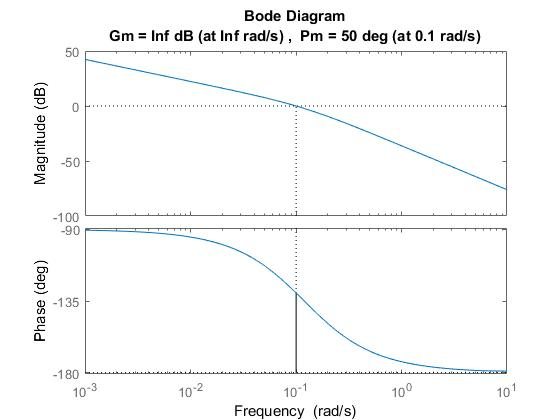
\includegraphics[width=1\textwidth]{Plots/3a_bode_plot.jpg}
    \caption{Bode Plot used to optimize our PD controller with $K_{pd} = 0.84$ and $T_f = 8.36$ giving $\omega_c = 0.10$ (rad/s) and phase margin = $50^{\circ}$}
    \label{fig: 3a_bode_plot}
\end{figure}

\begin{figure}[H]
    \centering
    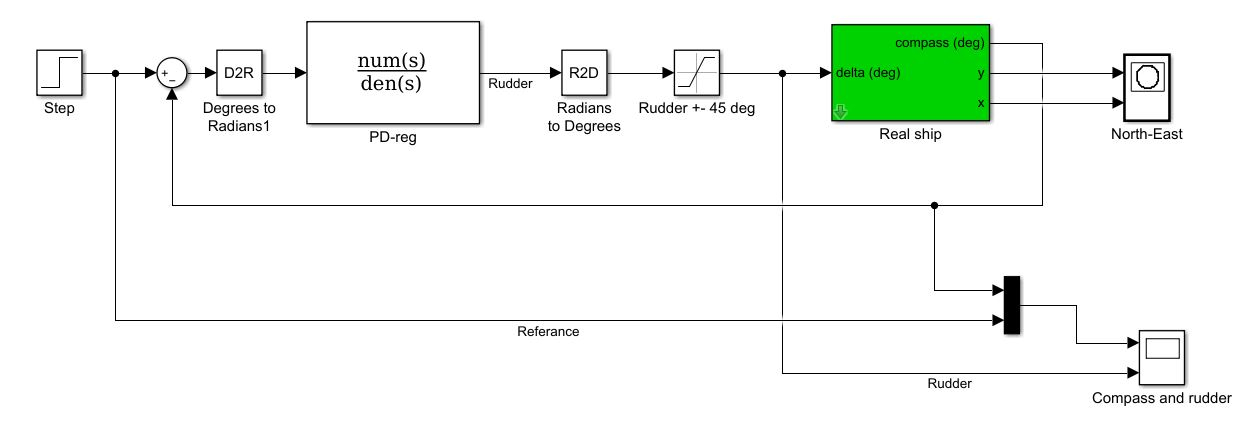
\includegraphics[width=1\textwidth]{Plots/3bcd_simulink_model.jpg}
    \caption{Simulink model with the PD controller implemented. Saturation block is added due to the rudders physical restrictions}
    \label{fig: 3bcd_simulink}
\end{figure}


\begin{figure}[H]
    \centering
    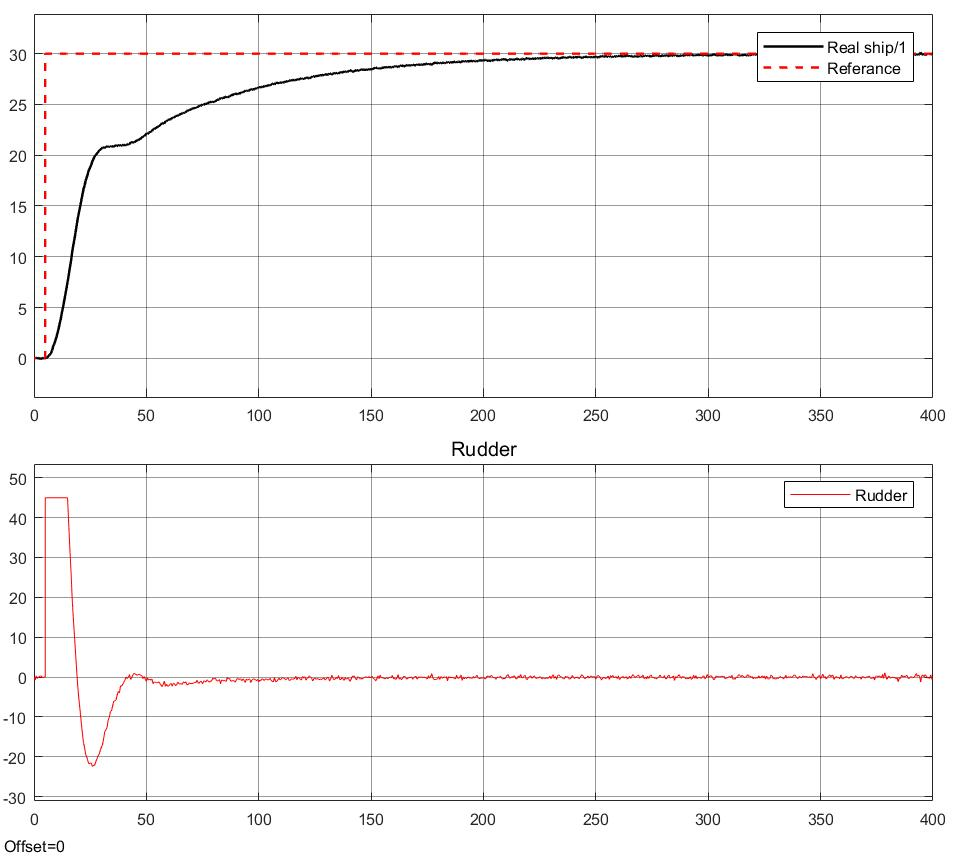
\includegraphics[width=1\textwidth]{Plots/3b_compass_and_ref.jpg}
    \caption{The plot shows the ship with autopilot using a PD-regulator. Only measurement noise is enabled.}
    \label{fig: 3b_plot}
\end{figure}

\begin{figure}[H]
    \centering
    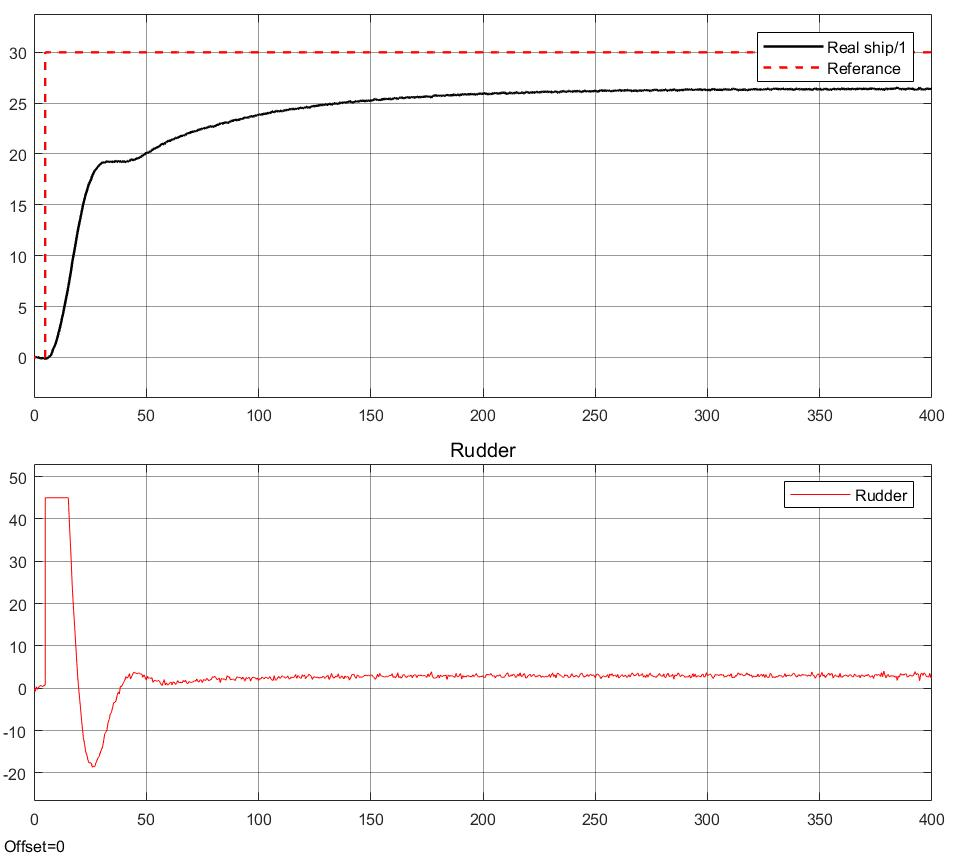
\includegraphics[width=1\textwidth]{Plots/3c_compass_and_ref.jpg}
    \caption{The plot shows the ship with autopilot using a PD-regulator. Measurement noise and current are enabled.}
    \label{fig: 3c_plot}
\end{figure}

\begin{figure}[H]
    \centering
    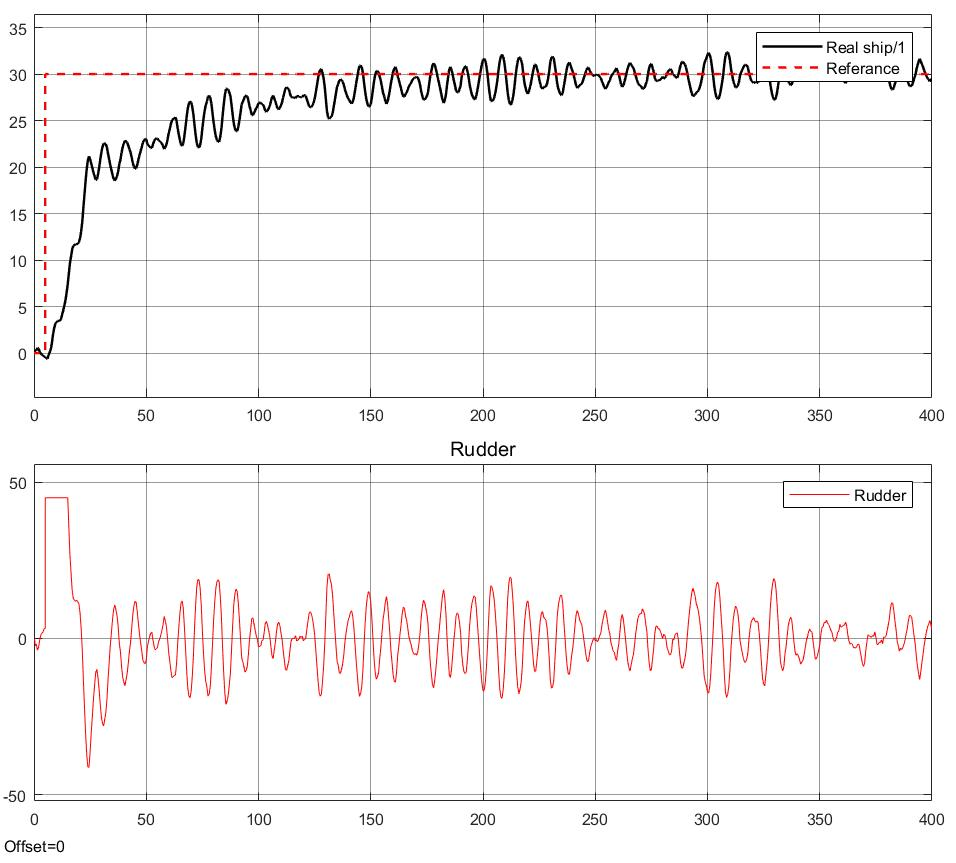
\includegraphics[width=1\textwidth]{Plots/3d_compass_and_ref.jpg}
    \caption{The plot shows the ship with autopilot using a PD-regulator. Measurement noise and waves are enabled.}
    \label{fig: 3d_plot}
\end{figure}